\addcontentsline{toc}{chapter}{Introduction}
\chapter*{Introduction}
Mathematical modeling and scientific computing is, now, an inseparable part of engineering and science, thanks to advances in computational science and technology. Models expressed as partial differential equations (PDEs) can be found in a wide range of disciplines from social sciences, biology, cosmology, modern and classical physics, and engineering to industrial applications. The overwhelming success of such models, in approximately describing the nature, has encouraged the development of complex mathematical models in order to attain higher accuracy. The complexity of many modern applications, however, is computationally prohibitive with classical approaches. The curse of dimensionality for multi-dimensional parameter sets, i.e. the exponential growth in computational costs in higher dimensions, is an example of a computational inefficiency that inhibits such approaches.

Reduced order modeling (ROM), apposed to high-fidelity modeling, has emerged as a successful attempt to reduce the intrinsic computational inefficiencies of modern applications. ROM aims to accurately represent the high-fidelity model with a few degrees of freedom, by exploiting empirical or physical structures in data. Confining the model to only these degrees of freedom can, then, significantly reduce the computational costs. Although these methods do not eliminate the need for high-fidelity modeling, however, they significantly accelerate the evaluation of outputs of interest when repeated computation of the high-fidelity model is required.

%Reduced basis (RB) methods, are a class of techniques for ROM, which restricts the high-fidelity model to a subspace with a, relatively, low dimension. Representing the high-fidelity model in this subspace, using a projection operator, reduces the system size of the system of algebraic equations that describe the model. 

Recognition of patterns in data, in general, makes ROM comparable with machine learning techniques, e.g. in computer science and statistics developed during the past decades. However, the deterministic nature of PDEs together with the control in the choice of data generation process, gives ROM a distinctive take on artificial intelligence. 

This difference, between ROM and conventional machine learning techniques, becomes more apparent with time-dependent problems. Time-symmetries of high-fidelity models are lost in the ensembling of data, which sometimes, result in an ill-represented ROM. Although this inaccuracy in representation is less evident for parabolic PDEs, ROM of hyperbolic PDEs, where symmetries are a fundamental feature, remains a challenge.

The main aim of this thesis is to find ROM techniques that capture time-symmetries in a system of PDEs. Conservation of such symmetries, not only results in a robust ROM, but also it helps with a construction of a meaningful reduced order model. Time, as a parameter, plays a crucial role in the existence and the conservation of symmetries. Therefore, this thesis puts a particular emphasis on the treatment of the time variable by studying systems that depend on no, or otherwise very small number of other parameters. This might, at first glance, sounds counter intuitive in the context ROM. However, isolation of time can provide a remarkable insight into the theory of ROM, and even into mathematical modeling. Nevertheless, The main results of this paper can naturally be extended to the parameter setting while gaining all the benefits from conservation of symmetries.

In what is left of this chapter, we discuss the difficulties involving treating time as a parameter in the context of ROM, and then, we briefly discuss the content of the thesis.

\section*{Space and Time in ROM}
Reduced basis (RB) methods are among the most popular ROM techniques. These methods has been successful in reducing the computational complexity of large scale systems of partial differential equations, and has been used in many disciplines in engineering and science and widely applied in industry. 

RB methods, is based on the assumption that a state of a solution to a system of PDEs can be well approximated by a few degrees of freedom, chosen from a low-dimensional subspace. A projection operator, often of a linear type, is then constructed, to confine the state of the system to this subspace. This constructs a new system of partial differential equations that now is described only by a few independent variables. In principle, this system can be evaluated at an accelerated rate, compared to the high-fidelity system.

In the context of finite element method (FEM), where a solution to PDE is described as a linear combination of basis functions, RB methods can be visually represented. Consider the equations governing a 1-dimensional wave in a periodic domain.
\begin{equation} \label{eq:ch1.1}
	\frac{\partial }{\partial t^2} u(t,x) + \frac{\partial }{\partial x^2} u(t,x) = 0, \quad x\in[0,1],
\end{equation}
together with some initial condition $u(t,x) = u_0(x)$. A general finite element discretization requires $u$ to be a linear combination of a total of $n$, time-independent, basis functions $\varphi_i(x)$ as
\begin{equation} \label{eq:ch1.2}
	u(x,t) \approx \sum_{i=1}^n c_i(t) \varphi_i(x),
\end{equation}
where $c_i(t)$ are the expansion coefficients, that determine the degrees of freedom. In this setting, the choice of $u_i$ is independent of the empirical setting of \eqref{eq:ch1.1}. Exploiting some problem-specific patterns, e.g., arising from initial and boundary conditions, problem geometry, or numerical properties, allows us to introduce a new, but smaller, set of basis functions $\psi_i$. Requiring
\begin{equation} \label{eq:ch1.3}
	u(x,t) \approx \sum_{i=1}^k c'_i(t) \psi_i(x),
\end{equation}
\begin{figure} [t]
	\subfloat[FEM basis functions\label{fig:ch1.1a}]{%
		\includegraphics[width=0.45\textwidth]{./images/intro/hat}
	}
	\subfloat[RB basis functions\label{fig:ch1.1b}]{%
			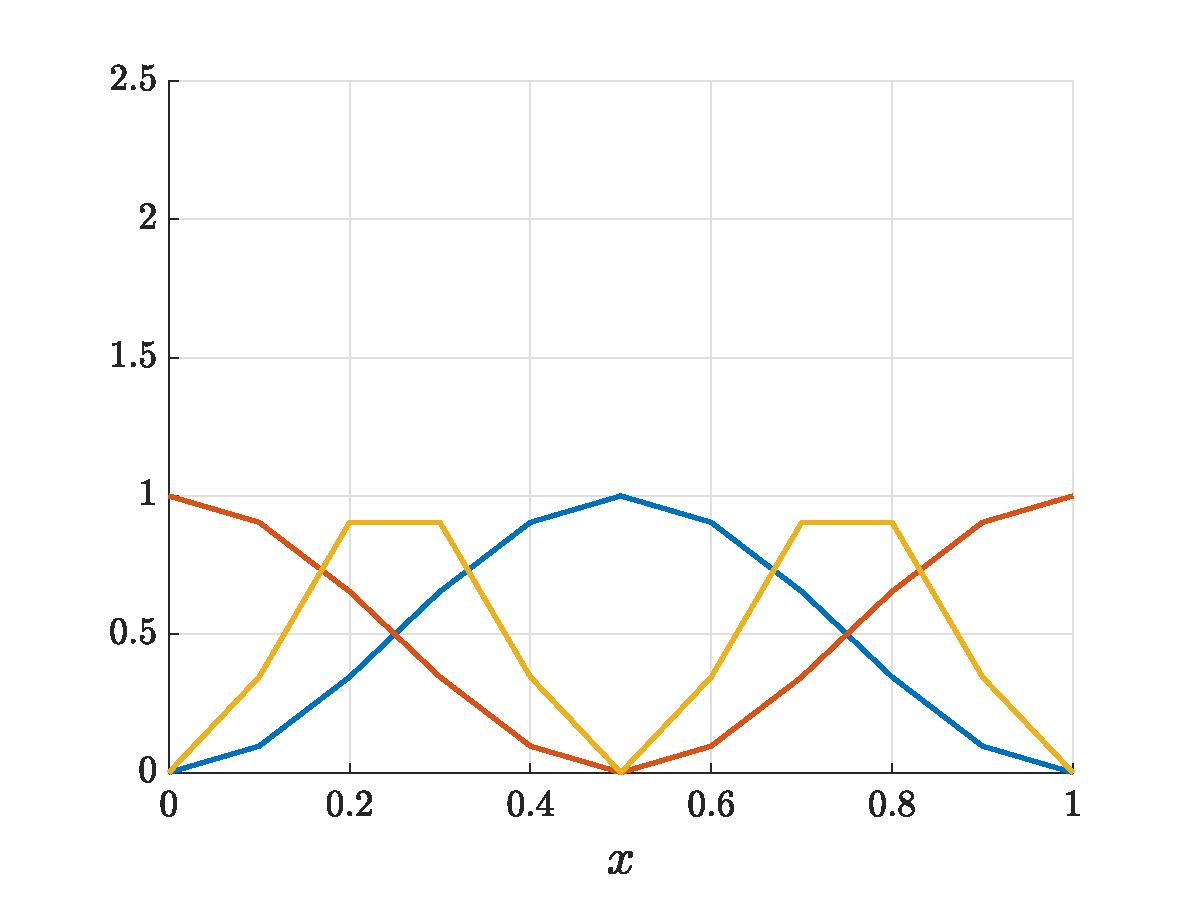
\includegraphics[width=0.45\textwidth]{./images/intro/pod}
	}
	\caption{spacial representation of MOR}
	\label{fig:ch1.1}
\end{figure}
can deliver the desired accuracy. Given $k \ll n$, we gain acceleration, in principle, in evaluating only $k$ coefficients rather $n$. Often, RB methods require the relation between $\psi_i$ and $\varphi_i$ to be a linear relation, i.e.
\begin{equation} \label{eq:ch1.3.1}
	\psi_i = \sum_{j=1}^n r_j \varphi_j, \quad i=1,\dots,k.
\end{equation}
A rough sketch of basis functions $\varphi_i$ and $\psi_i$ is seen in \Cref{fig:ch1.1}. This is a \emph{spacial perspective} of reduced order modeling.

To be able to visualize the temporal aspect of MOR, we simplify \eqref{eq:ch1.1}, to obtain an ordinary differential equation (ODE) $\ddot u(t) - u(t) = 0$, which can be written in the terms of first order ODEs as
\begin{equation} \label{eq:ch1.4}
	\left\{
	\begin{aligned}
		\dot u(t) &= v(t), \\
		\dot v(t) &= -u(t).
	\end{aligned}
	\right.
\end{equation}
Introduction of the new variable $v$ is not only an algebraic tool, but carries a deeper insight in the dynamics of the original second order ODE. For instance, $H(u,v) = u^2 + v^2$ is a constant quantity, and can be interpreted as the energy of \eqref{eq:ch1.4}. Therefore, the value of $v$ is restricted by $H$, in a nonlinear sense. Another insight into the dynamics of \eqref{eq:ch1.4} is revealed when we consider vector fields in the coordinate system $(u,v)$, commonly referred to as the \emph{phase space}. \Cref{fig:ch1.2a} shows the vectors fields $\nabla H$ and $(\dot u, \dot v)$. We immediately notice the orthogonality of the two vector fields. Periodic behaviour of \eqref{eq:ch1.4} is a result of this delicate relation. Such properties of \eqref{eq:ch1.4} that are unchanged along a trajectory are often referred to as \emph{symmetries} or \emph{time-symmetries} of \eqref{eq:ch1.4}.
\begin{figure} [t]
	\begin{centering}
	\subfloat[original vector fields\label{fig:ch1.2a}]{%
		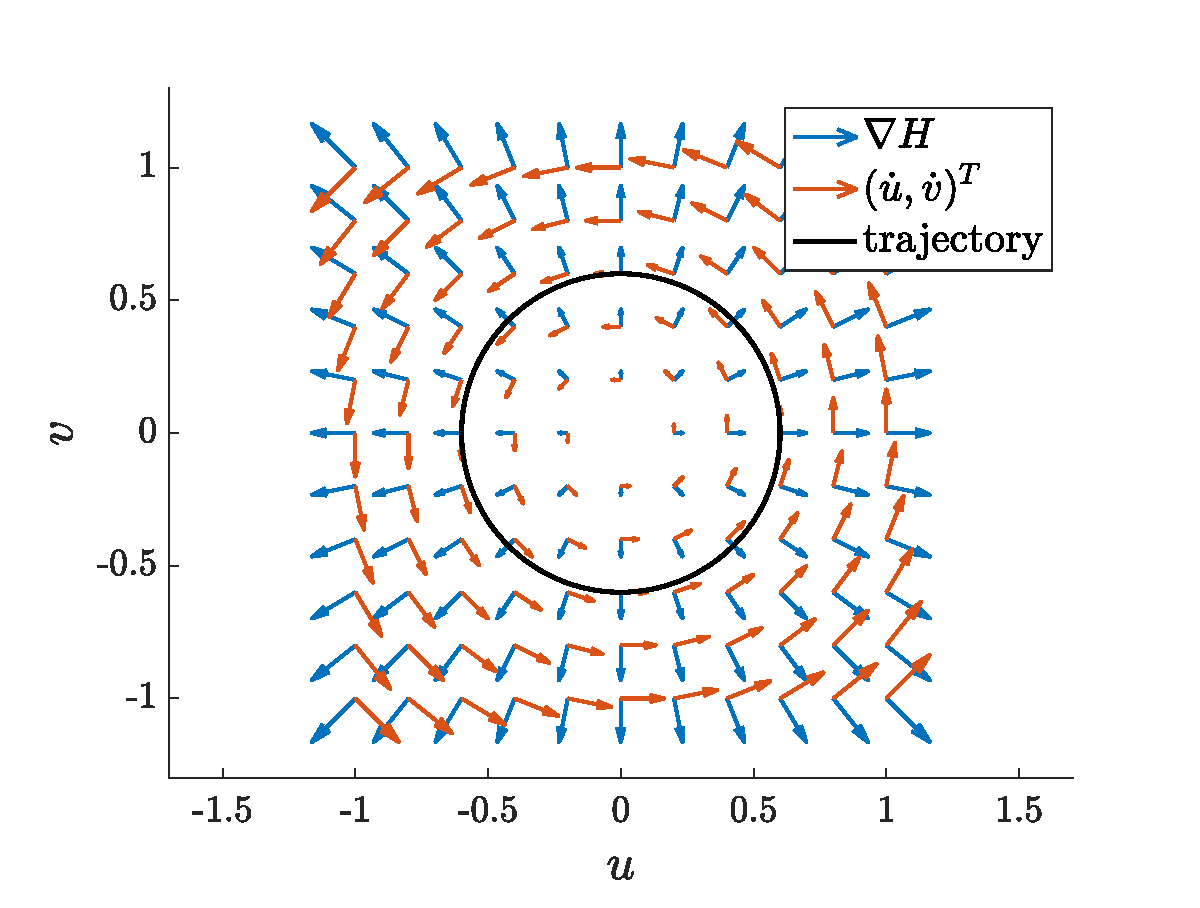
\includegraphics[width=0.45\textwidth]{./images/intro/orig}
	}
	\subfloat[transformation of vector fields\label{fig:ch1.2b}]{%
			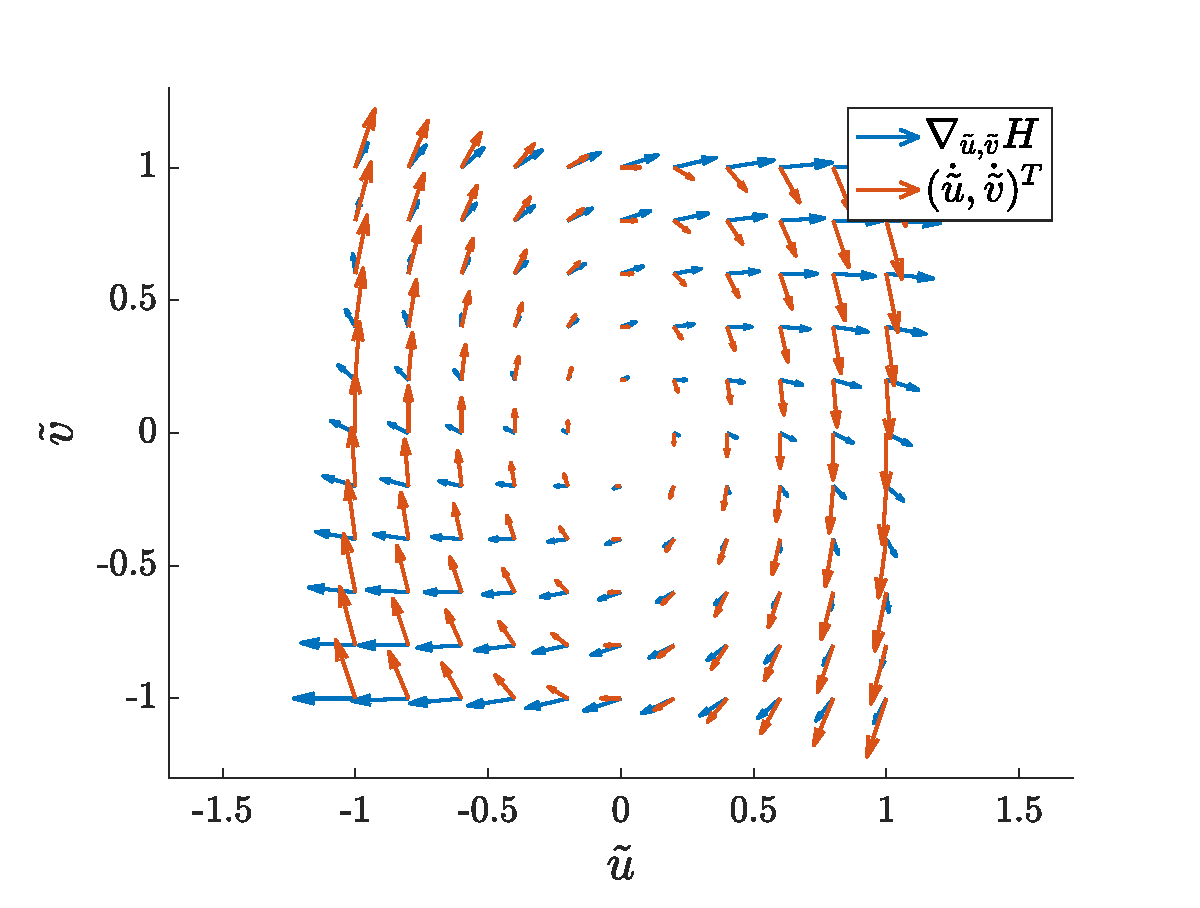
\includegraphics[width=0.45\textwidth]{./images/intro/trans}
	} \\
	\subfloat[symplectic transformation of vector fields\label{fig:ch1.2c}]{%
			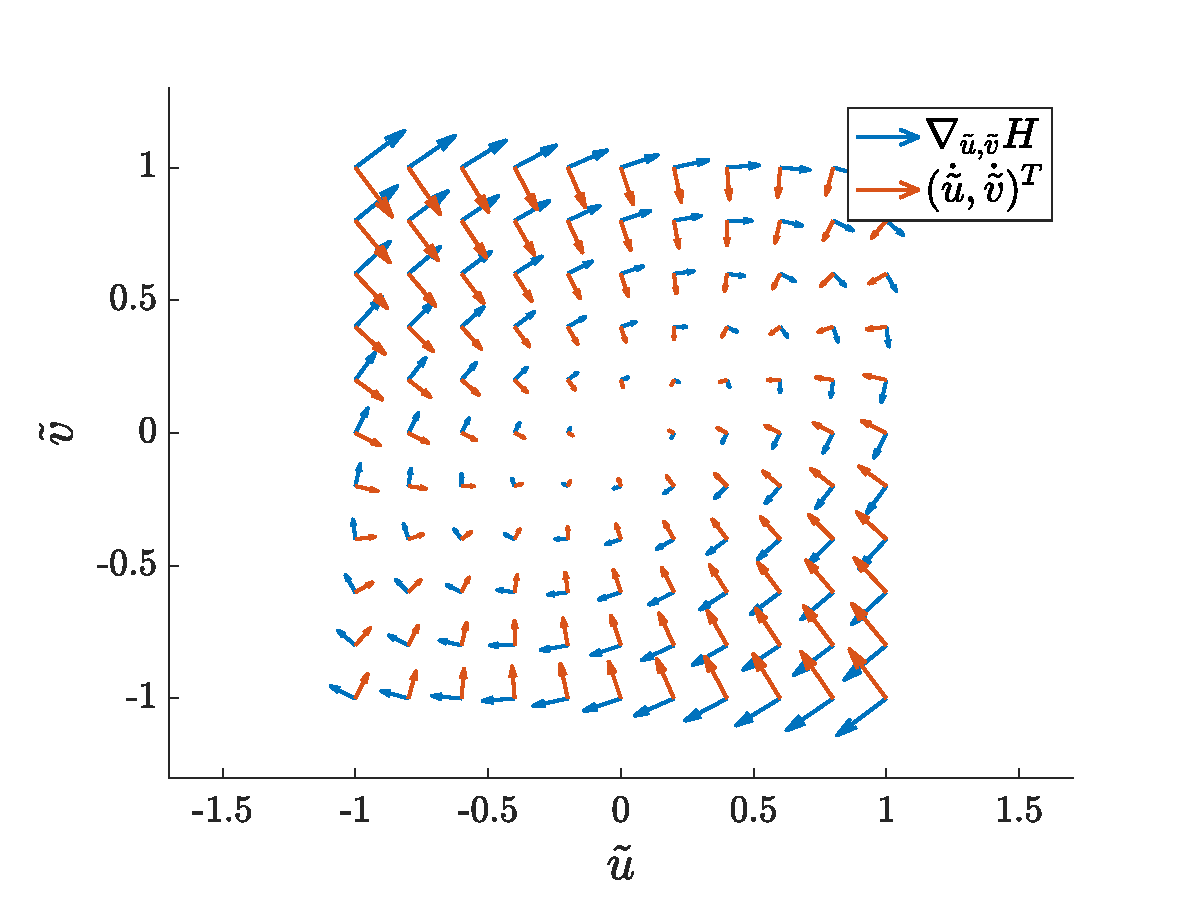
\includegraphics[width=0.45\textwidth]{./images/intro/symp}
	}
	\caption{temporal representation of MOR}
	\label{fig:ch1.2}
	\end{centering}
\end{figure}


Let us now study the symmetries of \eqref{eq:ch1.4} in a transformed coordinate system. \Cref{fig:ch1.2b} shows the transformation of $\nabla H$ and $(\dot u, \dot v)$ over some linear transformation $(\tilde u, \tilde v) = T(u,v)$. We notice that the orthogonality of the two the two vector fields is destroyed. Although, the dynamics of the original and the transformed system is the same, the transformed system is less symmetrical. For some class of linear transformations, \emph{symplectic transformations}, the orthogonality of the two vector fields is preserved. This can be seen in \Cref{fig:ch1.2c} where a linear symplectic transformation is applied to $\nabla H$ and $(\dot u, \dot v)$.

In a numerical approximation, loss of symmetries can have profound consequences for the overall dynamics of a system. For example, the trajectory of \eqref{eq:ch1.4}, which is a distinctive feature of the dynamics, can no longer remain periodic in a non-symmetrical coordinate system.

In the context of MOR, basis functions, e.g., those in \Cref{fig:ch1.1a}, can be viewed as a basis for the phase space. Subsequently, a solution expanded in this basis can be translated as a vector in the phase space. The relation \eqref{eq:ch1.3.1} is, therefore, interpreted as a change in the coordinate system. This is the \emph{temporal perspective} of MOR.  

Similar to \eqref{eq:ch1.4}, we can define similar orthogonal vectors fields for \eqref{eq:ch1.1} as $(\partial u/\partial t,\partial v/\partial t)$ and $\nabla H$ with $v = \partial u/\partial t$ and $H(u,v) = \int v^2 + (\partial u / \partial x)^2 \ dx$. Therefore, we expect a general RB method to result in a non-symmetrical phase space. Specially since the patterns in the ensemble of solution to \eqref{eq:ch1.1} does not reveal the subtle relation between the two vector fields.

Nonlinear invariants and symmetries, such as those discussed above, are a fundamental feature of hyperbolic system of PDEs. Loss of symmetries, in such systems, can explain the challenge in MOR of hyperbolic problems.

The main aim of this thesis is to seek RB techniques that construct a reduced phase space that captures the symmetries of the high-fidelity system of PDEs. This ensures conservation of some nonlinear invariants and, subsequently, well-approximation of the overall dynamics in the reduced system. Hamiltonian systems, as systems that are driven by symmetries, are studied intensively from MOR view point. We then develop methods that preserve symmetries of a fluid flow.

\section*{Overview of The Thesis}
The overall goal of this thesis is to investigate RB techniques that can preserve nonlinear invariants, symmetries, and conservation laws. Furthermore, it aims to understand the stability and robustness properties of these methods compared to conventional RB techniques. The main focus of this thesis is the MOR of time-dependent and, in particular, hyperbolic PDEs. A particular emphasis is put on model order reduction of Hamiltonian systems to fully understand the role of time in structure-preserving MOR. The main results are then generalized to construct a MOR method for fluid flow.

\Cref{chapter:2} surveys the background on smooth manifolds and Hamiltonian systems. We introduce the concept of geometrical symmetry and how it relates to the dynamics of a time-dependent differential equations. We also briefly introduce methods for conserving these symmetries in a numerical evaluation.

An overview on the theory of model order reduction is presented in \Cref{chapter:3}. We present conventional RB techniques, e.g. proper orthogonal decomposition and the greedy method, for generating a reduced basis. Galerkin and Petrov-Galerkin projection is then discussed for constructing a reduced system. This chapter discusses efficient evaluation of nonlinear terms with the introduction of the empirical interpolation method.

Symplectic MOR for Hamiltonian systems is introduced in \Cref{chapter:4}. It is discussed how symplectic transformations can be used to construct a reduced Hamiltonian system that preserves the dynamics of the high-fidelity Hamiltonian system. We present a greedy method for generation of a symplectic basis as well as other SVD-based symplectic model reduction techniques. Accuracy, stability, and efficiency of the method are discussed through numerical experiment.

In \Cref{chapter:5} we couple the symplectic model order reduction with a weighted inner-product. We show that this can be viewed as a natural generalization to the symplectic MOR. Numerical experiments are presented to illustrate how this method can be beneficial when an unstructured numerical discretization is used in the high-fidelity system.

\Cref{chapter:6} presents symplectic MOR in the context of dissipative Hamiltonian system. It is discussed how a canonical extension of dissipative Hamiltonian system yields a closed an conservative system. This chapter discusses how an application of a symplectic MOR on an extended system can help with a correct evolution of the Hamiltonian. Performance of this method is illustrated through simulation of the dissipative Hamiltonian and port-Hamiltonian systems.

A conservative model reduction of fluid flow is presented \Cref{chapter:7}. It is explained in this chapter how the skew-symmetry of differential operators in fluid flow can help recover conservation of quadratic invariants, e.g. energy, at the level of reduced system. It is discussed how this give rise to a physically meaningful reduced system with quadratic invariants with respect to reduced variables. Stability properties of the method is illustrated through various numerical experiments of incompressible and compressible fluid.
